\documentclass[11pt]{article}

\usepackage[T2A]{fontenc}
\usepackage[utf8x]{inputenc}

\usepackage[russian, english]{babel}

\usepackage{vmargin}
\setpapersize{A4}
\setmarginsrb{1cm}{1cm}{1cm}{1cm}{0pt}{0pt}{0mm}{13mm}

\usepackage{amssymb, amsmath}

\usepackage{graphicx}

\sloppy

\begin{document}
	\begin{enumerate}
		\section{Магнетизм}
		\item Причины возникновения магнитного поля.\\
		Магнитное поле создается движущимися зарядами.
		\item Основные характеристики магнитного поля.\\
		Силовыми характеристиками магнитного поля являются вектор \textbf{магнитной индукции (B)} и вектор \textbf{напряженности магнитного поля (H)}, показывающих направление линий магнитной индукций, густота этих линий пропорциональна модулю магнитной индукции, а касательная к ним в каждой точке поля показывает направление вектора магнитной индукции в этой точке.
		\item Проявление магнитного поля и механизмы на их основе\\
		\item Теорема о циркуляции вектора H\\
		Циркуляция вектора \textbf{H} по произвольному контуру $\Gamma$ равна аглебраической сумме токов, охватываемых контуром $\Gamma$:
		$$
			\oint_\Gamma H\, dl = I = \sum I_k
		$$
		\item Закон Био-Савара-Лапласа\\
		Для движущегося заряда:
		$$
			d\mathbf{B} = \frac{\mu\mu_0}{4\pi}\frac{[\mathbf{j, r}]dV}{r^3}
		$$
		Для тонкого провода:
		$$
			d\mathbf{B} = \frac{\mu\mu_0}{4\pi}\frac{I[d\mathbf{l, r}]}{r^3}
		$$
		\item Задача на нахождение B вблизи изогнутых проводов с током\\
		Ну, там удачи короче Вам с интегральчиками
		\item Сила Лоренца\\
		Сила, действующая на движущийся со скоростью $\mathbf{v}$ заряд $q$ со стороны магнитного поля $\mathbf{B}$ и равная $\mathbf{F}_\text{л} = q[\mathbf{vB}]$, называется \textit{силою Лоренца}.
		\item Задача на силу Лоренца\\
		Ну, тоже с векторами там провозитесь
		\item Сила Ампера\\
		Сила, действующая на со стороны магнитного поля $\mathbf{B}$ на проводник с током I, называют \textit{силою Ампера}. Элементарная сила Ампера $d\mathbf{F}$, действующая на малый элемент $dl$ длины проводника, по которому идет электрический ток I, равна:
		$$
			d\mathbf{F} = I[d\mathbf{lB}]
		$$
		\item Магнитный момент\\
		\item Сила, действующая на элементарный контур с током\\
		\item Момент сил, действующих на контур с током\\
		\item Магнитное поле в веществе (намагниченность)\\
		\item Магнетики (виды магнетиков, основные характеристики и графики, петля гистерезиса)\\
		\item Устройство постоянного магнита\\
		\item Электромагнитная индукция\\
		\textit{Явление электромагнитной индукции} состоит в том, что в проводящем контуре, находящемся в переменном магнитном поле, возникает \textit{электродвижущая сила индкукции} $\mathcal{E}_i$, если контур замкнут, то в нем возникает электрический ток, называемый \textit{индукционным током}.

		\textit{Закон электромагнитной индукции Фарадея:} э.д.с. электромагнитной индукции $\mathcal{E}_i$ в контуре численно равна и противоположна по знаку скорости изменения магнитного потока $\text{Ф}_m$ сквозь поверхность, ограниченную этим контуром:
		$$
			\mathcal{E}_i = -\frac{d\text{Ф}_m}{dt}
		$$
		\item Самоиндукция\\
		Возникновение э.д.с. индукции в цепи в результате изменения тока в этой называется \textit{явлением самоиндукции}. Собственное магнитное поле тока в контуре создает магнитный поток $\text{Ф}_{mc}$ сквозь поверхность S, ограниченную самим контуром:
		$$
			\text{Ф}_{mc} = \int_S B_n dS.
		$$
		Магнитный поток $\text{Ф}_mc$ называют \textit{потоком самоиндукции контура}. Если контур находится в неферромагнитной среде, то его поток самоиндукции пропорционален току I в контуре:
		$$
			\text{Ф}_{mc} = LI
 		$$
		\item Взаимная индукция, трансформаторы\\
		\item Задача на индукцию\\
		\item Электромагнитный колебательный контур\\
		\item Уравнения Максвелла в интегральной и дифференциальной форме\\
		\begin{description}
			\item[Первое уравнение Максвелла]
			\begin{align}
				\oint_L (\mathbf{E}d\mathbf{l}) = -\frac{\partial\text{Ф}_m}{\partial t}\\
				\mathbf{\nabla\times E} = -\frac{\partial\mathbf{B}}{\partial t}
			\end{align}
			\item[Второе уравнение Максвелла]
			\begin{align}
				\oint_L (\mathbf{H}d\mathbf{l}) = \sum_{k=1}^n I_k + I_\text{смещ}\\
				\mathbf{\nabla\times H} = \mathbf{j} + \frac{\partial\mathbf{D}}{\partial t}
			\end{align}
			\item[Третье уравнение Максвелла]
			\begin{align}
				\text{Ф}_e = \oint_S D_n dS = q,\\
				\mathbf{\nabla\cdot D} = \rho
			\end{align}
			\item[Четвертое уравнение Максвелла]
			\begin{align}
				\text{Ф}_m = \oint_S B_n dS = 0,\\
				\mathbf{\nabla\cdot B} = 0
			\end{align}
			\item[Материальные уравнения]
			\begin{align}
				\mathbf{D} &= \varepsilon\varepsilon_0\mathbf{E} & \mathbf{B} &= \mu\mu_0\mathbf{H} & \mathbf{j} &= \gamma\mathbf{E} 
			\end{align}
		\end{description}
	\end{enumerate}
	\begin{enumerate}
		\section{Геометрическая оптика}
		\item Зеркала. Построение изображений в двух зеркалах.
			\paragraph{Определение}
			\textbf{Зеркало} ~--- гладкая поверхность, предназначенная для отражения света (или другого излучения).
			\paragraph{Виды зеркал}
			\begin{itemize}
				\item Сферические
				\item Плоские
			\end{itemize}
			\paragraph{Сферическое зеркало}
			\textbf{Сферическое зеркало} ~--- зеркало, отражающая поверхность которого имеет вид сегмента сферы.
			\paragraph{Описание}
			Сферическое зеркало может быть выпуклым или вогнутым ~--- в зависимости от того, какая сторона сегмента сферы ~--- выпуклая или вогнутая ~--- является отражающей. Центр соответствующей сферическому зеркалу сферы называется его центром или оптическим центром, середина сегмента ~--- полюсом зеркала, прямая, проходящая через центр и полюс ~--- главной оптической осью зеркала. Другие прямые, проходящие через центр зеркала и точку, отличную от полюса, называются его побочными оптическими осями.

			Параксиальные лучи, параллельные главной оптической оси выпуклого сферического зеркала, так же как и продолжения параксиальных лучей, параллельных главной оптической оси вогнутого сферического зеркала, пересекаются в одной точке, называемой его фокусом. Он расположен посередине между центром и полюсом зеркала, то есть расстояние (F) его до зеркала равно половине радиуса (R): 
			$$
				F = \frac{R}{2}
			$$

			У сферического зеркала, как вообще у любого зеркала, отсутствует хроматическая аберрация, но выражена сферическая аберрация. Сферическая аберрация выражена потому, что в отличие от параболического зеркала (то есть сегмента параболоида вращения), сферическое зеркало может собирать в одной точке лишь параксиальные лучи, то есть те из лучей, параллельных главной оптической оси, которые близки к этой оси. Сферическая аберрация в одном из примеров применения сферического вогнутого зеркала, зеркально-линзовом телескопе системы Дмитрия Максутова, устраняется компенсированием специально подобранной линзой ~--- мениском.

			Известным примером выпуклого сферического зеркала является ёлочный шар.
			\paragraph{Ход лучей в сферическом зеркале}
			Проще всего построить изображение отрезка, перпендикулярного главной оптической оси зеркала и настолько небольшого по высоте, что луч, исходящий из его верхней точки и параллельный главной оптической оси зеркала — параксиальный. Его изображение будет также перпендикулярным главной оптической оси зеркала, расстояние его от зеркала при известном расстоянии от зеркала до предмета и фокусного расстояния зеркала можно вычислить по формуле зеркала. Высота изображения $(h')$ будет равна произведению высоты предмета $(h)$ на отношение расстояния от изображения до зеркала $(f)$ к расстоянию от зеркала до предмета $(d)$:
			$$
				h' = h\cdot\frac{f}{d}
			$$
			\paragraph{В вогнутом (впуклом) сферическом зеркале}
			Если сферическое зеркало вогнутое, возможны различные случаи расположения изображения относительно зеркала при различных расстояниях до предмета. Буквой $C$ обозначен центр зеркала, а буквой $F$ ~--- его фокус. При $d>F$ формула зеркала имеет вид:
			$$
				\frac{1}{d} + \frac{1}{f} = \frac{1}{F},
			$$
			а при $d < F$
			$$
				\frac{1}{d} - \frac{1}{f} = \frac{1}{F}
			$$
			Для построения взято три луча (хотя достаточно и двух):
			\begin{itemize}
				\item луч, параллельный главной оптической оси после отражения от зеркала пройдёт через его фокус;
				\item луч, проходящий через фокус после отражения пойдёт параллельно главной оптической оси;
				\item луч, падающий на полюс зеркала после отражения пойдёт под углом, равным углу падения (по закону отражения света).
			\end{itemize}
			\begin{figure}[!ht]
				\minipage{0.25\textwidth}
					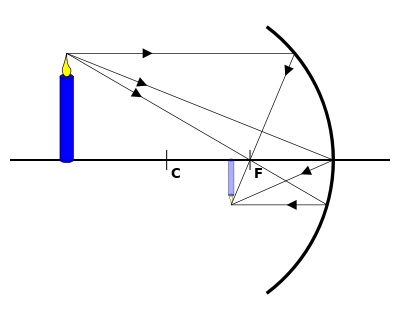
\includegraphics[width=\linewidth]{assets/mirrors/sphere_mirror1.png}
				\endminipage\hfill
				\minipage{0.25\textwidth}
					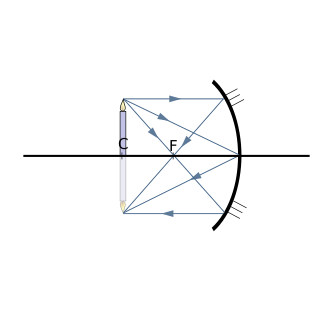
\includegraphics[width=\linewidth]{assets/mirrors/sphere_mirror2.png}
				\endminipage\hfill
				\minipage{0.25\textwidth}
					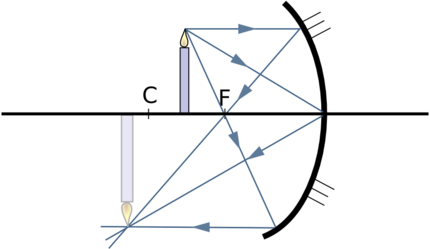
\includegraphics[width=\linewidth]{assets/mirrors/sphere_mirror3.png}
				\endminipage\hfill
				\minipage{0.25\textwidth}
					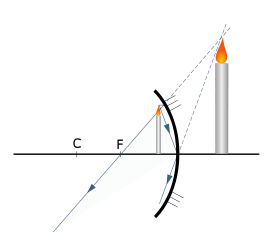
\includegraphics[width=\linewidth]{assets/mirrors/sphere_mirror4.png}
				\endminipage
			\end{figure}
			\paragraph{В выпуклом (выгнутом) сферическом зеркале}
			Построение изображения в выпуклом сферическом зеркале проще, чем в вогнутом: здесь при любом расстоянии предмета до зеркала его изображение будет расположено за зеркалом. На рисунке ниже буквой F обозначен фокус выпуклого зеркала, буквой V — полюс, y (в формуле u) — высота предмета, y' (в формуле v) — высота изображения. Формула зеркала в этом случае имеет вид:
			$$
				\frac{1}{u} - \frac {1}{v} = -\frac{1}{F}
			$$
			Для построения взято два луча:
			\begin{itemize}
				\item луч от верхней точки предмета, параллельный главной оптической оси, отразится от зеркала, и продолжение этого отражённого луча пройдёт через фокус и через верхнюю точку изображения;
				\item луч от верхней точки предмета, продолжение которого проходит через фокус, после отражения пойдёт параллельно главной оптической оси, а продолжение этого отражённого луча также пройдёт через верхнюю точку изображения.
			\end{itemize}

			Таким образом, верхней точкой изображения будет точка пересечения продолжения первого отражённого луча и продолжения второго отражённого луча.
			\begin{figure}[!ht]
				\centering
				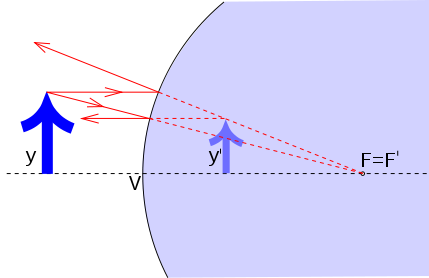
\includegraphics[width=0.5\textwidth]{assets/mirrors/sphere_mirror5.png}
			\end{figure}
			\paragraph{Плоское зеркало}
			\textbf{Плоское зеркало} ~--- зеркало, отражающая поверхность которого имеет вид плоскости.
			\paragraph{Ход лучей в плоском зеркале}
			Принцип хода лучей, отражённых от зеркала, прост, если применять законы геометрической оптики, не учитывая волновую природу света. Пусть луч света падает на идеальную плоскую зеркальную поверхность, полностью отражающую весь падающий на него свет, под некоторым углом к нормали (перпендикуляру), проведённой к поверхности в точке падения луча на зеркало. Тогда отражённый луч будет лежать в плоскости, образованной падающим лучом и нормалью к поверхности, а угол, образованный отражённым лучом и нормалью, будет равен углу падения. Луч, падающий на зеркало под прямым углом к плоскости зеркала, отразится сам в себя.
			\begin{figure}[!ht]
				\centering
				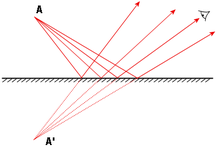
\includegraphics[width=0.5\textwidth]{assets/mirrors/plane_mirror.png}
			\end{figure}
			Для простейшего ~--- плоского ~--- зеркала изображение будет расположено за зеркалом симметрично предмету относительно плоскости зеркала, оно будет мнимым, прямым и такого же размера, как сам предмет. Это нетрудно установить, пользуясь законом отражения света. Плоское зеркало также можно рассматривать как предельный случай сферического зеркала (неважно, выпуклого, или вогнутого), при радиусе, стремящемся к бесконечности, тогда его свойства получаются из формулы сферического зеркала и формулы увеличения сферического зеркала.
			\paragraph{Построение изображений в двух плоских зеркалах}
			Для начала запишем формулу числа изображений в двух плоских зеркалах расположенных под углом $\alpha$:
			$$
				N = \frac{360^\circ}{\alpha} - 1
			$$
			В качестве примера рассмотрим систему двух зеркал, установленных под углом $90^\circ$.
			Свеча $A$ находится между двумя зеркалами, образующими двугранный прямой угол.
			\begin{figure}[!ht]
				\centering
				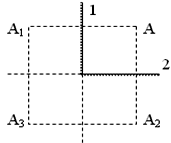
\includegraphics[width=0.5\textwidth]{assets/mirrors/two_mirrors1.png}
			\end{figure}

			Сколько изображений свечи дают зеркала и где эти изображения расположены? Ответ пояснить с помощью рисунка.

			Два изображения $A_1$ и $A_2$ расположены симметрично точке $A$ относительно зеркал 1 и 2. Эти мнимые изображения образованы лучами, отразившимися от одного из зеркал. Но часть лучей, отразившись сначала от зеркала 1, отражается затем и от зеркала 2. После первого отражения пучок этих лучей как бы исходит из точки $A_1$ (в этой точке пересекаются их продолжения). Значит, после второго отражения появится еще мнимое изображение $A_3$ точки $A_1$ в зеркале 2. Изображение точки $A_2$ в зеркале 1 тоже попадает в точку $A_3$. Более двух отражений не испытывает ни один луч; следовательно, других изображений нет. Это видно из того, что точка $A_3$ уже не может отразиться от какого-либо зеркала: для обоих зеркал она находится в «зазеркалье». 
			\begin{figure}[!ht]
				\centering
				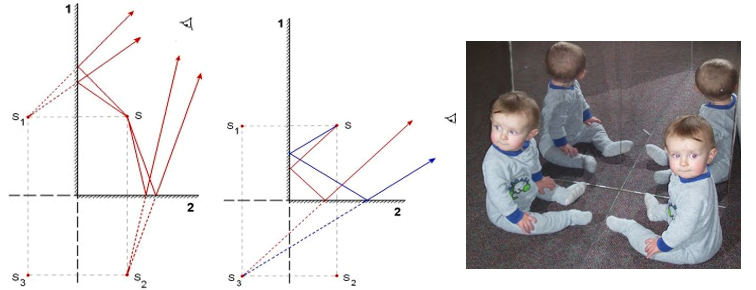
\includegraphics[width=0.5\textwidth]{assets/mirrors/two_mirrors2.png}
			\end{figure}
		\item Общий вывод поворота отраженного луча при повороте зеркала.
		Пусть начальный поворот зеркала к горизонтали, угол падения и угол отражения равны соответственно $\alpha_1, \beta_1, \varphi_1$, тогда имеет место следующее соотношение $\alpha_1 = \beta_1$. Пусть зеркало повернули на угол $\varphi_2$, тогда угол падения и угол отражения стали соответственно $\alpha_2 = \beta_2$. Очевидно, что насколько повернулось зеркало настолько и повернулся перпендикуляр к нему, тогда по построению видно, что $\alpha_2 = \alpha_1 + \Delta\varphi = \alpha_1 + \varphi_2 - \varphi_1$. Изначально угол между падающим и отраженным был $\Delta_1 = \alpha_1 + \beta_1 = 2\alpha_1$, после поворота он стал $\Delta_2 = \alpha_2 + \beta_2 = 2\alpha_2$. Получается, что отраженный луч повернулся на $\Delta = \Delta_2 - \Delta_1 = 2\cdot (\alpha_2 - \alpha_1) = 2\cdot\Delta\varphi$. Ч.Т.Д.
		\item Линзы. Два основных принципа построения в тонкой линзе (пример применения).
		\section{Волновая оптика}
		\section{Интерференция}
		\section{Дифракция}
		\section{Поляризация}
		\section{Квантовая физика}
		\section{История развития представлений об атоме}
	\end{enumerate}
\end{document}